\begin{center}
\shorthandoff{<>}
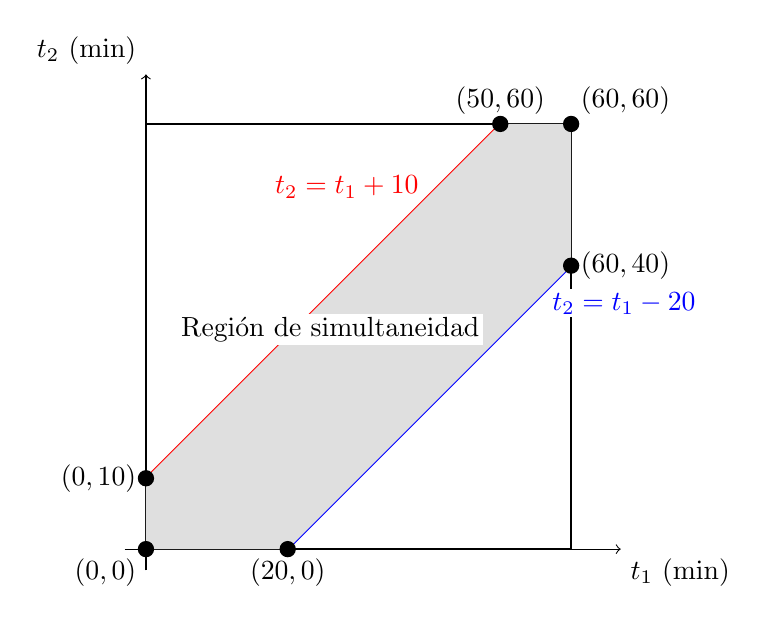
\begin{tikzpicture}[scale=0.09]
  % axes
  \draw[->] (-3,0) -- (67,0) node[below right] {$t_1$ (min)};
  \draw[->] (0,-3) -- (0,67) node[above left] {$t_2$ (min)};

  % support square
  \draw[thick] (0,0) rectangle (60,60);

  % boundary lines of the band
  \draw[blue, thick] (20,0) -- (60,40)
    node[pos=0.92, below right, fill=white, inner sep=1pt] {$t_2=t_1-20$};
  \draw[red, thick] (0,10) -- (50,60)
    node[pos=0.78, above left, fill=white, inner sep=1pt] {$t_2=t_1+10$};

  % feasible region: (0,0)-(20,0)-(60,40)-(60,60)-(50,60)-(0,10)
  \fill[gray!25] (0,0) -- (20,0) -- (60,40) -- (60,60) -- (50,60) -- (0,10) -- cycle;

  % vertices
  \foreach \x/\y in {0/0,20/0,60/40,60/60,50/60,0/10}{
    \fill (\x,\y) circle (1.15);
  }

  % vertex labels (offset to avoid overlap)
  \node[below left]  at (0,0)   {$(0,0)$};
  \node[below]       at (20,0)  {$(20,0)$};
  \node[right]       at (60,40) {$(60,40)$};
  \node[above right] at (60,60) {$(60,60)$};
  \node[above]       at (50,60) {$(50,60)$};
  \node[left]        at (0,10)  {$(0,10)$};

  % region label
  \node[fill=white, inner sep=1.2pt] at (26,31) {Región de simultaneidad};
\end{tikzpicture}
\shorthandon{<>}
\end{center}